\documentclass[24pt]{article}
\usepackage{physics}
\usepackage{graphicx}
\usepackage{listings}
\usepackage{color}

\definecolor{dkgreen}{rgb}{0,0.6,0}
\definecolor{gray}{rgb}{0.5,0.5,0.5}
\definecolor{mauve}{rgb}{0.58,0,0.82}

\lstset{frame=tb,
  language=Python,
  aboveskip=3mm,
  belowskip=3mm,
  showstringspaces=false,
  columns=flexible,
  basicstyle={\small\ttfamily},
  numbers=none,
  numberstyle=\tiny\color{gray},
  keywordstyle=\color{blue},
  commentstyle=\color{dkgreen},
  stringstyle=\color{mauve},
  breaklines=true,
  breakatwhitespace=true,
  tabsize=3
}



\begin{document}


\title{Simulating realistic falling bodies in Python}
\author{Sahil Islam}
\date{}
\maketitle

\section*{The Theory}
Hopefully we all heard about the famous Galileo's Leaning Tower of Pisa experiment
where he drops two spherical objects from the top of the leaning tower of Pisa, and 
calculates the time taken by them to reach the ground. From there he concluded that, if there is no air resistance(or negligible one), multiple bodies with equal masses will take the same time to fall from a high alltitude. And if there is sygnificant resistance, the time will depend on the masses of the bodies. \\
Here we don't have acces to the leaning tower of Pisa. SO, we are going to simlate that using a programming language called Python. But first we need to know or better formulate the theory.\\
To formulate this let's first take one body and analyze what happens if we leave it  from a position higher than a ground. We all know what happens, it falls down. But why? that is the question. According to the great Newton and his Gravitational theory, every particle having a mass in the universe attracts another (particle having a mass) with a particular force, the gravitational force. And if no other force balances this gravitaional force, the particles(or masses) starts accelerating. The magnitude of the force is: \\

$\va{F}=-G \frac{m_1 m_2}{r^2} \vu{r} $
\\

Here $m_1$ and $m_2$ are the masses of the bodies and $r$ is the distance between them. And the direction of the force is along -ve $ \vu{r}$ . This force is always attractive.(G here is called Universal Gravitational constant.)\\
Now here on earth, all the objects, living/non living are attracted by the earth with a force that follows the above formula. If we take the mass of the earth as $M$ and radius be $R$ and distance of the body at a height $h$ from the surface of the earth, then the gravitaional force on the body of mass $m$ is \\

$\va{F}=- G \frac{M m}{(R+h)^2} \vu{R}$\\

Thus it's evident that the force has a direction opposite to $\vu{R}$ which is measured from the centre of the earth. Thus $\va{F}$ has s direction towards the centre of the earth. Thus everything falls on the ground.\\
Now this force gives the body an acceleration. We call it Gravitational Acceleration. We can find the acceleration by dividing the force with mass of its own. Thus the magnitude of the gravitaional acceleration is:\\
$g= G\frac{M}{(R+h)^2}$\\

At the surface of the earth i.e. $h=0$ we can find the $g= 9.8 ms^{-1}$ by putting the values of mass and radius of the earth.Though it's evident from the equation that g changes with $h$, but this change is not that much, so we will take $g=9.8$ for now.\\
Thus if any body falls from some height, it falls with the acceleration $g$ which does not depend on its mass. That means no matter how heavy or light the object  we release from the Pisa, both of them will have the same acceleration.\\
We can find out the time taken by them to reach the ground very easily. We know, the accleration means the change of velocity over time, and the velocity means the change of poition over time. In terms of calculus this is written as:\\

$a=\dv{v}{t}$ and $v=\dv{x}{t}$\\

Here $a$, $v$ and $x$ are acceleration, velocity and position of object and $t$ is the time.
Here we know the acceleration is $g$. So:\\

$\dv{v}{t}=g$\\

Integrating this we can write:\\

$v(t)=v(t=0)+gt$\\

Here $v(t=0)$ is the velocity at $t=0$, in this case it is 0. So,\\

$v(t)=gt$\\

$\Rightarrow \dv{x(t)}{t}=gt$\\

Integrating again, we get:\\

$x(t)=\frac{1}{2} g t^2 + x(t=0)$\\

Here $x(t=0)$ is the height from where we are releasing the bodies.\\
Now if we release the objects at a height $h$ and if they take $\tau$ time to rach the ground, then:\\
$x(t=0)=0$ and $x(t=\tau)=h$\\

Thus we get, \\

$\tau=\sqrt{\frac{2 h}{g}}$\\

Hence, we see that time taken by two bodies to fall from a particular height dows not depend on their mass, size or anything else. It just depends on the gravitational acceleration and the height from where it's been released.

This is a beautiful phenomenon, though it is not that realistic. Because in real nature, there is a air drag effect , which may caus\\
***********INCOMPLETE****************

\section*{The Computation}
As I promised, we are going to compute this. SO, let's see how to do this.\\
We will use a very beautiful python module called 'pygame' to visualize this. And ofcourse we will do this in 2D. \\
 The core logic is, we will define a circle on the canvas which has pa particular x and y position. This x and y position will change according to the x and y velocity, and this x and y velocity will change according to the x and y acceleration. Here in this case the objects will not have any x velocity, the will only have velocity in the y deirection, and acceleration in the y direction which is $g$. The diagram should help: \\
\begin{figure}[h!]
\centering
	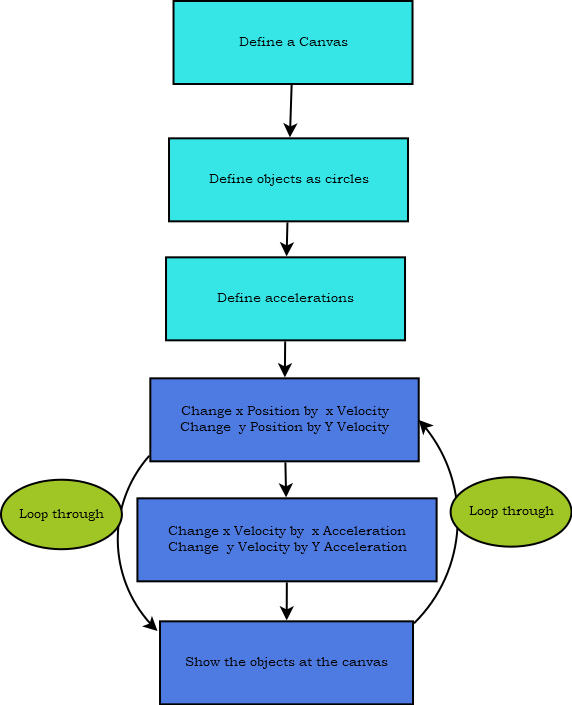
\includegraphics[width=0.5\textwidth]{fallingBodies.png}
	\caption{Algorithm}
\end{figure}\\





Now let's see the code:\\
\begin{lstlisting}


"""Code simulates falling balls with air drag proportional to velocity square."""

### Sahil Islam ###
### 16/06/2020 ###

import pygame
import numpy as np

pygame.init()
width = 800
height = 650
screen = pygame.display.set_mode((width, height))
surface = pygame.Surface((width, int(height / 2.)))
white = (255, 255, 255)
black = (0, 0, 0)
red = (255, 0, 0)
blue = (0, 0, 255)
lightblue = (153, 217, 234)
clock = pygame.time.Clock()


def ball(x, y, m):
    r = m  # Radius and mass are made proportional for visual understanding.
    pygame.draw.circle(screen, black, (int(x), int(y)), r, 2)


def drag(cd, v, m):
    a = float(cd * v * v) / m
    return a


g = 9.8
c = 1.1

no_of_balls = 5
xPos = np.random.randint(20, width - 20, no_of_balls)
mass = np.random.randint(10, 50, no_of_balls)
yPos = np.zeros(no_of_balls)

xVel = np.zeros(no_of_balls)
yVel = np.zeros(no_of_balls)

xAcc = np.zeros(no_of_balls)
yAcc = np.zeros(no_of_balls)

dt = 0.1  # Time step for better prcession.

while True:

    screen.fill(white)
    surface.fill(lightblue)
    screen.blit(surface, (0, int(height / 2.) ))
    for i in range(len(xPos)):

        ball(xPos[i], yPos[i], mass[i])

        yAcc[i] = +g - drag(0, yVel[i], mass[i])

        if yPos[i] + mass[i] >= height / 2.0:
            yAcc[i] = +g - drag(c, yVel[i], mass[i])

        xPos[i] += dt * xVel[i]
        yPos[i] += dt * yVel[i]
        xVel[i] += dt * xAcc[i]
        yVel[i] += dt * yAcc[i]

        if yPos[i] + mass[i] >= height:
            yVel[i] *= 0
            xVel[i] *= 0

        for event in pygame.event.get():
            if event.type == pygame.QUIT:
                pygame.quit()
                quit()

    pygame.display.update()
    clock.tick(50)

\end{lstlisting}


\end{document}